%%%%%%%%%%%%%%%%%%%%%%%%%%% asme2ej.tex %%%%%%%%%%%%%%%%%%%%%%%%%%%%%%%
% Template for producing ASME-format journal articles using LaTeX    %
% Written by   Harry H. Cheng, Professor and Director                %
%              Integration Engineering Laboratory                    %
%              Department of Mechanical and Aeronautical Engineering %
%              University of California                              %
%              Davis, CA 95616                                       %
%              Tel: (530) 752-5020 (office)                          %
%                   (530) 752-1028 (lab)                             %
%              Fax: (530) 752-4158                                   %
%              Email: hhcheng@ucdavis.edu                            %
%              WWW:   http://iel.ucdavis.edu/people/cheng.html       %
%              May 7, 1994                                           %
% Modified: February 16, 2001 by Harry H. Cheng                      %
% Modified: January  01, 2003 by Geoffrey R. Shiflett                %
% Use at your own risk, send complaints to /dev/null                 %
%%%%%%%%%%%%%%%%%%%%%%%%%%%%%%%%%%%%%%%%%%%%%%%%%%%%%%%%%%%%%%%%%%%%%%

%%% use twocolumn and 10pt options with the asme2ej format
\documentclass[twocolumn,10pt]{asme2ej}

\usepackage[utf8]{inputenc}
\usepackage{mathtools}
\usepackage{amsmath}
\usepackage{graphicx}
\usepackage[italian]{babel}

\newcommand{\abs}[1]{\left|#1\right|}

%% The class has several options
%  onecolumn/twocolumn - format for one or two columns per page
%  10pt/11pt/12pt - use 10, 11, or 12 point font
%  oneside/twoside - format for oneside/twosided printing
%  final/draft - format for final/draft copy
%  cleanfoot - take out copyright info in footer leave page number
%  cleanhead - take out the conference banner on the title page
%  titlepage/notitlepage - put in titlepage or leave out titlepage
%  
%% The default is oneside, onecolumn, 10pt, final


\title{Predizione della struttura di una proteina (PSP) in un lattice 2D}

\author{Emanuele Carraro}

\begin{document}

\maketitle    

%%%%%%%%%%%%%%%%%%%%%%%%%%%%%%%%%%%%%%%%%%%%%%%%%%%%%%%%%%%%%%%%%%%%%%
\begin{abstract}
{\it Il problema di predizione della struttura terziaria di una proteina è molto rilevante nell'ambito della bioinformatica, infatti la configurazione assunta nello spazio determina le sue proprietà biologiche.

Di seguito vengono analizzati tre metodi di risoluzione del problema, uno tramite ricerca informata (algoritmo hill-climbing), uno tramite la definizione di un problema con vincoli e, infine, uno con un noto algoritmo di reinforcement learning (Q-learning).
}
\end{abstract}

%%%%%%%%%%%%%%%%%%%%%%%%%%%%%%%%%%%%%%%%%%%%%%%%%%%%%%%%%%%%%%%%%%%%%%
\begin{nomenclature}
\entry{PSP}{Protein structure prediction}
\entry{$\mathcal{E}_c$}{Matrice dell'energia di una proteina}
\entry{H}{Amminoacido idrofobico}
\entry{P}{Amminoacido polare}
\end{nomenclature}

\section{Background}

Una proteina è un complesso biologico di macromolecole composte da \textbf{sequenze di amminoacidi}.

Gli amminoacidi vengono uniti durante la sintesi proteica grazie alla creazione di un legame peptidico (figura \ref{fig:pept}).

\begin{figure}[h]
\centering
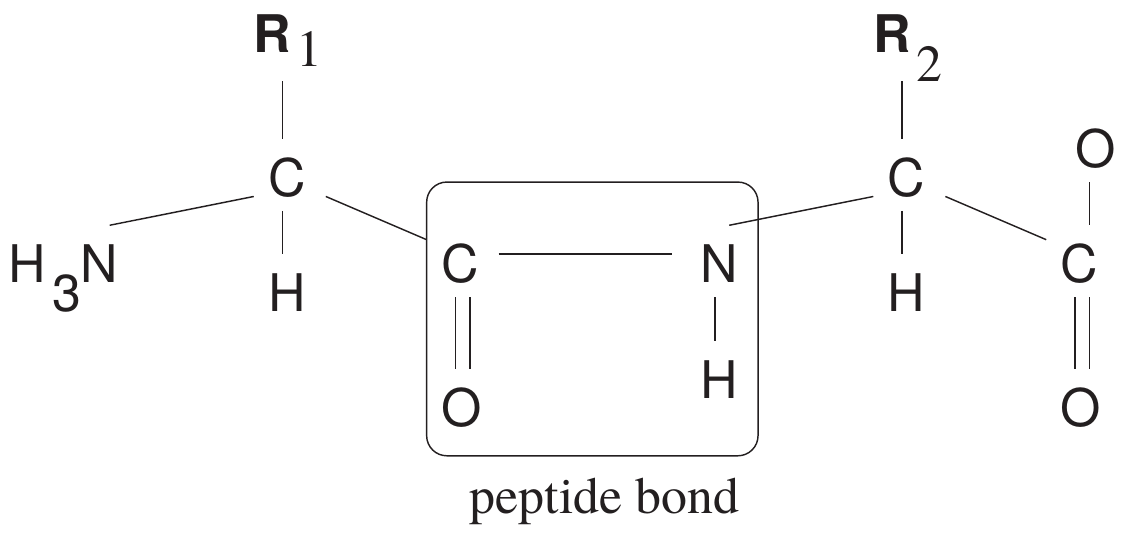
\includegraphics[width=0.4\textwidth]{figure/peptideBond.png}
\caption{Legame peptidico}
\label{fig:pept}
\end{figure}

La \textbf{struttura primaria} di una proteina è data dalla pura sequenza di amminoacidi e condiziona la configurazione spaziale e la forma globale della molecola.

L'avvolgimento a spirale e la disposizione regolare di tratti più o meno lunghi della catena proteica costituiscono la \textbf{struttura secondaria}.\\

Di solito, gruppi di queste strutture secondarie si combinano fra loro per formare la \textbf{struttura terziaria}, dalla quale dipendono le proprietà biologiche della molecola. La predizione della struttura di una proteina (PSP) è quindi una sfida molto importante nell'ambito della biologia molecolare.

Tutte le tecniche computazionali di predizione assumono che la struttura primaria di una proteina determini completamente la sua struttura terziaria (anche se nella realtà ci sono alcune eccezioni).

I modelli basati sulla struttura \textit{lattice} (o reticolo) si sono dimostrati utili per ragionare a proposito della complessità di questo problema. Un modello con lattice porta a ``discretizzare'' lo spazio di configurazione di una proteina e può essere classificato in base a determinate proprietà:

\begin{enumerate}
 \item Come viene rappresentata la struttura di una proteina (ad esempio, tramite un grafo)?
 \item Quale alfbeto di amminoacidi viene utilizzato (tutti i 20 conosciuti oppure solo 2 categorie - (H) idrofobi o (P) polari)?
 \item Quale formula utilizzare per descrivere l'\textbf{energia di una conformazione} (equivalente a una funzione di costo in un problema di ottimizzazione)?
 \item Che tipo di lattice scegliere (ad esempio, un lattice quadratico - 2D - o cubico - 3D)?
\end{enumerate}

\subsection{Il modello HP}

Uno dei modelli più usati è il modello HP: il lattice usato semplifica la struttura primaria di una proteina in un grafo, dato da una catena di nodi (gli amminoacidi) collegati da archi (i legami peptidici). Ogni nodo è un amminoacido che può essere di 2 tipi: H (idrofobico) o P (polare).
Questo modello riduce una proteina a una stringa composta dai caratteri ``H'' e ``P''. In questo modello le proteine tendono a raggruppare i nodi H attorno a un punto (cioè gli amminoacidi idrofobici formano un ``nucleo'') mentre i nodi P rimangono esterni.

Nella seguente notazione per semplicità si denota H con 1 e P con 0. Una proteina è dunque una sequenza binaria. L'energia usata in questo modello è data dal numero di ``contatti'' tra H (1). Se due amminoacidi H si trovano su punti adiacenti del lattice, allora contribuiscono di un'unità (negativa) all'energia.
Formalmente, sia $\mathcal{E}_c$ la matrice quadrata associata all'energia di una configurazione c di una sequenza binaria s di dimensioni ($|s|\cdot|s|$)

\begin{equation}
    \mathcal{E}_c = (e(a,b))_{a,b \in s} =
    \begin{cases*}
      -1 & if a = b = 1 \\
      0  & altrimenti
    \end{cases*}
\end{equation}

\subsection{Complessità computazionale del problema}

La ricerca esaustiva nello spazio delle possibili configurazioni di una proteina non è una soluzione algoritmica efficiente (non opera in tempo polinomiale) in quanto il numero di possibili configurazioni cresce esponenzialmente in relazione alla lunghezza della proteina.

Eppure, in natura il processo di ``folding'' (ripiegamento) di una proteina accade velocemente (impiega secondi o qualche minuto). L'ipotesi più accreditata è che una proteina assuma la configurazione con energia minima.

Di conseguenza, dato un modello di lattice L e una sequenza s, l'obiettivo è trovare una configurazione di s senza cicli in L che minimizzi l'energia.

\subsection{Modello square lattice}

Un reticolo a quadrato (square lattice) è un lattice a 2 dimensioni sugli interi ($Z^2$). Considerando un modello square lattice, l'impostazione del problema rimane la stessa, con il vincolo che gli amminoacidi/nodi del grafo debbano essere posizionati solo nei punti del reticolo.

Fornire un upper bound rispetto all'energia è un passo utile nello studio di questo modello. Si cerca qual è il numero massimo di contatti per una configurazione. Sia s una sequenza binaria e siano $\mathcal{P}[s]$ il numero di 1 in posizioni pari e $\mathcal{D}[s]$ il numero di 1 in posizioni dispari.

Dato che questo modello di lattice è bipartito, ogni 1 in posizione pari può avere un contatto con un 1 in posizione dispari. Sia $\mathcal{X}[s] = min\{\mathcal{P}[s], \mathcal{D}[s]\}$.

In ogni conformazione, il numero di contatti che può avere un 1 nella sequenza che non sia nè all'inizio nè alla fine, è 2 (altrimenti sarebbero 3). Quindi, il numero massimo di contatti in una configurazione di s nel reticolo quadrato è: $2 \mathcal{X}[s] + 2$

\begin{figure}[h]
\centering
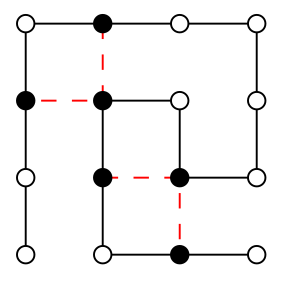
\includegraphics[width=0.3\textwidth]{figure/optConfig}
\caption{Una configurazione ottima per la sequenza 0010100001011010. I punti neri rappresentano 1 (H) mentre i punti bianchi 0 (P). Questa configurazione ha 4 contatti (linee tratteggiate) quindi l'energia totale è -4. L'upper bound per il numero massimo di contatti in questa sequenza è 2*2 + 2 = 6 ($\mathcal{X}[s] = 2$) \dots questo rappresenta un upper bound sul numero di contatti, non l'ottimo}
\label{fig:optConfig}
\end{figure}

\section{Problema con vincoli}

Data la struttura primaria di una proteina di lunghezza n, un problema tramite vincoli si definisce nel seguente modo:

\begin{enumerate}
 \item ciascun amminoacido viene assegnato a un punto sul reticolo 2D di dimensione $n \cdot n$ ($(x_i, y_i) \in Z^2$ $\forall i \in 1,..,n$, le coordinate i-esime appartengono all'amminoacido i-esimo);
 \item punti successivi nella struttura primaria non possono essere a una distanza maggiore di 1 tra loro ($\abs{x_i - x_{i+1}} + \abs{y_i - y_{i+1}} = 1 $ $\forall i \in 1,..,n-1$);
 \item due amminoacidi distinti non possono essere assegnati allo stesso punto sul reticolo ($ \neg (x_i = x_j \land y_i = y_j)$ $\forall i,j \in 1,..,n$).
\end{enumerate}

L'insieme di queste condizioni fa sì che il problema con vincoli ritorni l'intero insieme di configurazioni ammissibili della proteina nel reticolo 2D. Molte di queste sono ``simmetriche'', ossia la configurazione rimane la stessa ma la catena viene ``srotolata'' al contrario. Nella valutazione delle soluzioni non si tiene conto di queste simmetrie. Il problema così definito ritorna un insieme numeroso di soluzioni, esponenziale rispetto alla dimensione dell'input.

\section{Hill climbing search}

La hill climbing search necessita di:

\begin{enumerate}
 \item una soluzione iniziale (una configurazione ammissibile random);
 \item un modo per rappresentare una soluzione (in questo caso una soluzione è una sequenza di H,P);
 \item una definizione di vicinato (come ci si sposta da una soluzione a una sua ``vicina''?)
 \item una funzione che valuti le soluzioni (viene usata l'\textbf{energia di una configurazione});
 \item una strategia di esplorazione (viene usata la \textbf{best-first}).
\end{enumerate}

La definizione di vicinato in questo caso ha una forte componente randomica: data una soluzione, la struttura viene ``rotta'' in un punto casuale tra l'inizio e la fine della configurazione e da quel punto si scelgono mosse diverse (randomiche), determinando così il vicino. In questo modo, se il punto di taglio viene scelto all'inizio, gran parte della configurazione viene persa (al contrario, la maggior parte viene mantenuta).

\section{Reinforcement Learning}

Un task di reinforcement learning è composto da:

\begin{enumerate}
 \item lo spazio degli stati $\mathcal{S}$
 \item lo spazio delle azioni $\mathcal{A}$
 \item la funzione di transizione $\sigma$ che mappa una coppia (stato, azione) a uno dei probabili stati successori
 \item la funzione di ricompensa
\end{enumerate}

%Gabriela Czibula, Maria-Iuliana Bocicor and Istvan-Gergely Czibula

%%%%%%%%%%%%%%%%%%%%%%%%%%%%%%%%%%%%%%%%%%%%%%%%%%%%%%%%%%%%%%%%%%%%%%
% The bibliography is stored in an external database file
% in the BibTeX format (file_name.bib).  The bibliography is
% created by the following command and it will appear in this
% position in the document. You may, of course, create your
% own bibliography by using thebibliography environment as in
%
% \begin{thebibliography}{12}
% ...
% \bibitem{itemreference} D. E. Knudsen.
% {\em 1966 World Bnus Almanac.}
% {Permafrost Press, Novosibirsk.}
% ...
% \end{thebibliography}

% Here's where you specify the bibliography style file.
% The full file name for the bibliography style file 
% used for an ASME paper is asmems4.bst.
%\bibliographystyle{asmems4}

% Here's where you specify the bibliography database file.
% The full file name of the bibliography database for this
% article is asme2e.bib. The name for your database is up
% to you.
%\bibliography{asme2e}

\end{document}
